\documentclass{beamer}
\usetheme{metropolis}
\usepackage{subcaption}

% Configuration des couleurs modernes
\definecolor{myblue}{RGB}{173, 216, 230} % Bleu pastel
\definecolor{mymagenta}{RGB}{238, 130, 238} % Magenta doux
\definecolor{mywhite}{RGB}{255, 255, 255} % Blanc pur
\definecolor{mygray}{RGB}{245, 245, 245} % Gris clair
\definecolor{darkblue}{RGB}{25, 25, 112} % Bleu foncé
\definecolor{darkviolet}{RGB}{148, 0, 211} % Violet foncé
\definecolor{goldenrod}{RGB}{218, 165, 32} % Or doux

% Arrière-plan sobre et clair
\usepackage{tikz}

\addtobeamertemplate{background canvas}{}{
	\begin{tikzpicture}[remember picture, overlay]
		\fill[mywhite] (current page.south west) rectangle (current page.north east);
		\begin{scope}[blend mode=overlay]
			\shade[inner color=myblue!60, outer color=mywhite] (current page.south west) rectangle (current page.north east);
			\shade[inner color=mymagenta!60, outer color=mywhite] (current page.north east) rectangle (current page.south west);
		\end{scope}
	\end{tikzpicture}
}

% Personnalisation des couleurs dans metropolis
\setbeamercolor{normal text}{fg=black}
\setbeamercolor{frametitle}{bg=mywhite, fg=black}
\setbeamercolor{title separator}{fg=mymagenta}
\setbeamercolor{progress bar}{fg=myblue, bg=mymagenta}
\setbeamercolor{block title}{bg=myblue, fg=black}
\setbeamercolor{block body}{bg=mywhite, fg=black}
\setbeamercolor{alerted text}{fg=darkviolet!70}

% Personnalisation des typos
\setbeamerfont{frametitle}{size=\Large,series=\bfseries}
\setbeamerfont{title}{size=\Huge,series=\bfseries}

% Apparence des transitions entre les frames
\metroset{progressbar=frametitle,numbering=fraction}

% Commande pour ajuster le séparateur du titre
\metroset{titleformat frame=smallcaps}

% Début du document
\begin{document}
	
	\title{Diffusion Model}
	\subtitle{Machine Learning pour Physicien - Projet}
	\author{Clément, Grégoire, Nathan}
	\date{\today}
	
	\maketitle
	
	\section{Modèle de diffusion}
	
	\begin{frame}{Présentation générale}
		
		Les modèles de diffusion permettent de générer des images distribuées \alert{de la même manière} qu'un dataset donnée.
		
		\begin{figure}
			\centering
			\begin{subfigure}[b]{0.4\textwidth}
				\centering
				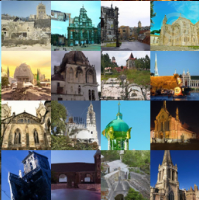
\includegraphics[scale=0.36]{imgs/Church_dataset.png}
				\caption*{Dataset}
			\end{subfigure}
			\begin{subfigure}[b]{0.4\textwidth}
				\centering
				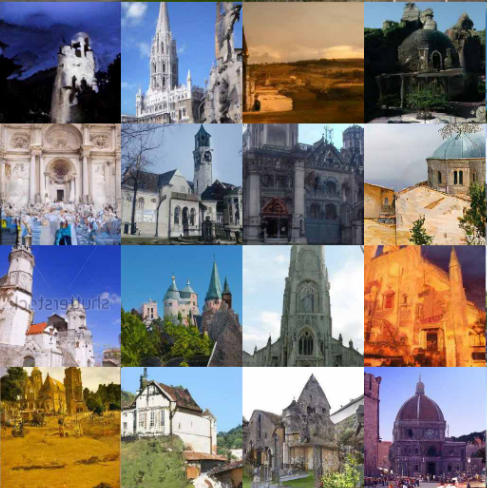
\includegraphics[scale=0.15]{imgs/Church_generated.png}
				\caption*{Images générées}
			\end{subfigure}
			\hfill
			\caption{Source : Denoising Diffusion Probabilistic Models, Ho. and Al.}
		\end{figure}
		
	\end{frame}
	
	\begin{frame}{Application en physique}
		Eliot si tu peux rajouter quelques trucs ici, genre des exemples avec des images
	\end{frame}
	
	\section{Denoising Diffusion Probabilistic Models, théorie}
	
	\begin{frame}{General Idea}
		\only<1>{Consider the set of \alert{hand-written digits $D$}. Can you give a probability distribution $q$ such that \alert{$x \sim q(x)$ ?}
			\begin{figure}
				\centering
				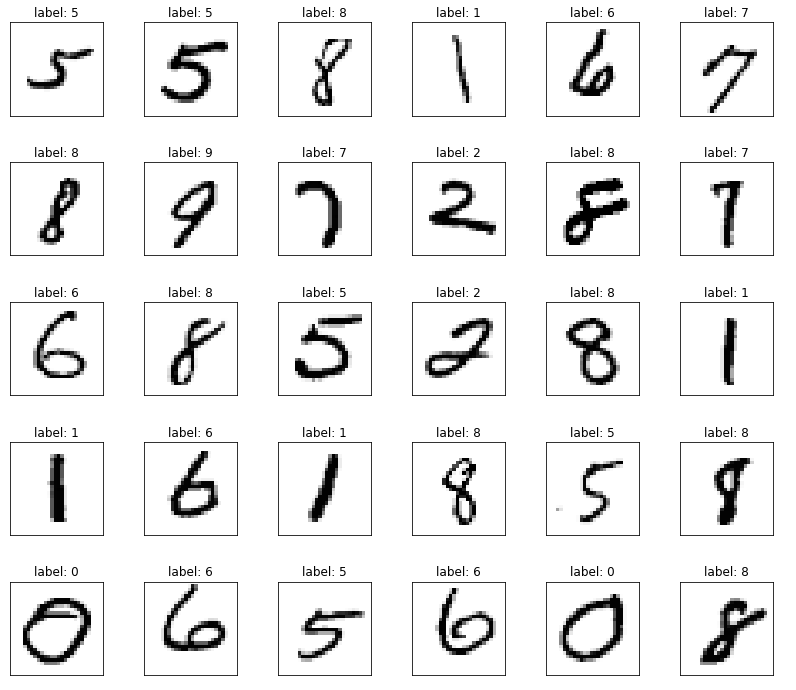
\includegraphics[width=0.5\textwidth]{imgs/mnist_sample_digits.png}
				\caption{Source: ludwig.ai}
			\end{figure}
		}
		\only<2->{
			Consider the set of \alert{hand-written digits $D$}. It is hard to find $q$ such that \alert{$x \sim q(x)$}, we need a \alert{clever way to sample hand-written digits}. Consider the following process:
			\begin{figure}
				\centering
				\begin{minipage}{0.2\textwidth}
					\centering
					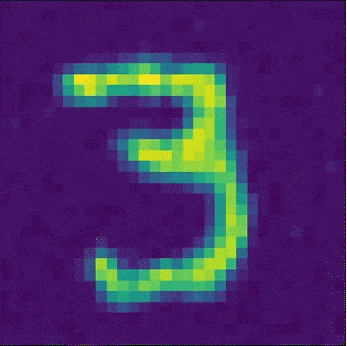
\includegraphics[width=\textwidth]{imgs/frame1.png}
				\end{minipage}%
				\only<3->{
					\begin{minipage}{0.2\textwidth}
						\centering
						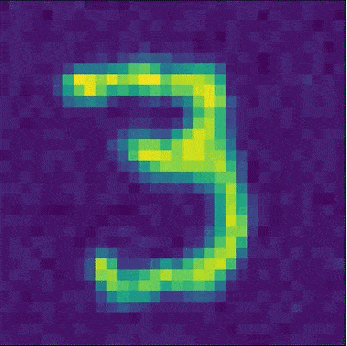
\includegraphics[width=\textwidth]{imgs/frame2.png}
					\end{minipage}
					\only<4->{
						\begin{minipage}{0.2\textwidth}
							\centering
							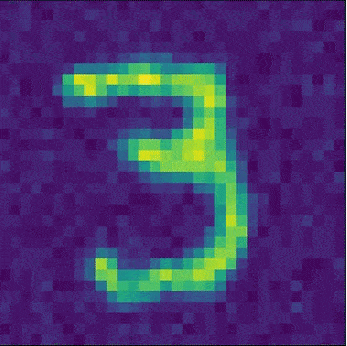
\includegraphics[width=\textwidth]{imgs/frame3.png}
						\end{minipage}
						\only<5->{
							\begin{minipage}{0.2\textwidth}
								\centering
								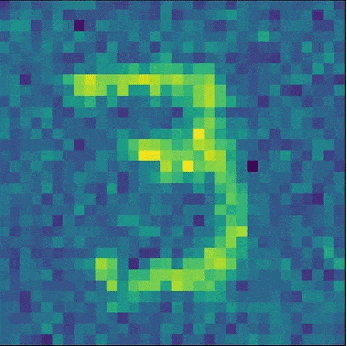
\includegraphics[width=\textwidth]{imgs/frame52.png}
							\end{minipage}
							\only<6->{
								\begin{minipage}{0.2\textwidth}
									\centering
									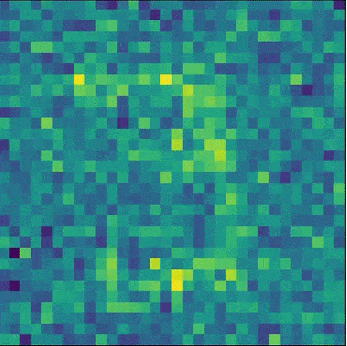
\includegraphics[width=\textwidth]{imgs/framelot.png}
								\end{minipage}
								\only<7->{
									\begin{minipage}{0.2\textwidth}
										\centering
										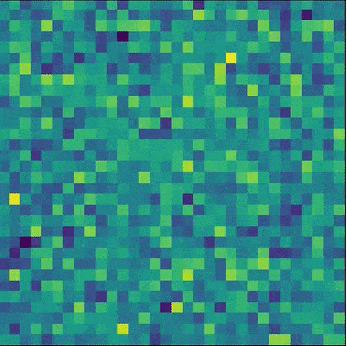
\includegraphics[width=\textwidth]{imgs/framerandom.png}
									\end{minipage}
								}
							}
						}
					}
					
				}
			\end{figure}
			\only<8->{
				Formally: $q(x_{t+1} \mid x_t) := \mathcal{N}(x_{t+1}; \sqrt{1 - \beta_t} x_t, \beta_t I)$ for some schedule $(\beta_t)_t$. Can we \alert{learn to reverse this process} ?
			}
		}
	\end{frame}
	
	
	
	\begin{frame}{What we want to learn}
		Given a noisy image $x_t$, we \alert{train a model to predict $x_{t-1}$}.
		\begin{figure}
			\centering
			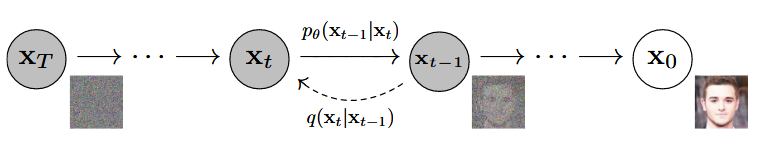
\includegraphics[width= \textwidth]{imgs/ho_diffusion_process.png}
		\end{figure}
		
		\only<2->{
			\begin{itemize}
				\item{Given a \alert{data image $x_0$}, we sample $(x_t)_{1:T}$ according to $q(x_{1:T} \mid x_0) := \prod_{t=1}^T q(x_t \mid x_{t-1})$,}
				\only<3->{\item{Given a \alert{noisy image $x_t$} and $t$, we sample according to $p_\theta (x_{t-1} \mid x_t) := \mathcal{N}(x_{t-1} ; \mu_\theta(x_t,t), \Sigma_\theta (x_t,t))$}.}
			\end{itemize}
		}
	\end{frame}
	
	\begin{frame}{Decreasing training data generation cost}
		Given a data image $x_0$, compute $x_t$ takes \alert{$t$ sampling on $q$}. But a \alert{simple trick}, allows to do only one.
		\uncover<2->{ 
			
			Remember that $q(x_{t+1} \mid x_t) := \mathcal{N}(x_{t+1}; \sqrt{1 - \beta_t} x_t, \beta_t I)$. Let $\alert{\alpha_t} = 1 - \beta_t$ and $\alert{\bar{\alpha_t}} = \prod_{i=1}^t \alpha_i$.
			\only<3-7>{
				\begin{align}
					x_t &= \sqrt{\alpha_t} x_{t-1} + \sqrt{1 - \alpha_t} \epsilon_{t-1} \nonumber\\
					\uncover<4->{
						&= \sqrt{\alpha_t} \sqrt{\alpha_{t-1}} x_{t-2} + \sqrt{\alpha_t} \sqrt{1 - \alpha_t} \epsilon_{t-1} + \sqrt{1 - \alpha_t} \epsilon_{t-1} \nonumber\\
						\uncover<6->{
							&= \sqrt{\alpha_t \alpha_{t-1}} x_{t-2} + \sqrt{\alpha_t(1 - \alpha_{t-1}) + 1 - \alpha_t} \bar{\epsilon_t} \label{eq:toexplain}\\ 
							\uncover<7->{
								&= \sqrt{\alpha_t \alpha_{t-1}} x_{t-2} + \sqrt{1 - \alpha_t \alpha_{t-1}} \bar{\epsilon_t} \nonumber
							}
						}
					}
				\end{align}
				\uncover<5-7>{Let $G_1 \sim \mathcal{N}(0,\sigma_1^2 I)$, $G_2 \sim \mathcal{N}(0,\sigma_2^2 I)$ , the sum of them gives $g_2 \sim \mathcal{N}(0,(\sigma_1^2 + \sigma_2^2) I)$.}
			}
			\only<8>{
				
				We have \alert{$x_t = \sqrt{\bar{\alpha_t}}x_0 + \sqrt{1 - \bar{\alpha_t}} \epsilon$}.
			}
		}
	\end{frame}
	
	\begin{frame}{Training}
		\only<1>{
			For now, our model is learning $\mu$ and $\Sigma$, i.e. we sample according to 
			\begin{align*}
				p_\theta (x_{t-1} \mid x_t) := \mathcal{N}(x_{t-1} ; \mu_\theta(x_t,t), \Sigma_\theta (x_t,t))
			\end{align*}
			They've found that \alert{fixing $\Sigma_\theta$} to a constant gives the same result. So,}
		\begin{align*}
			p_\theta (x_{t-1} \mid x_t) := \mathcal{N}(x_{t-1} ; \mu_\theta(x_t,t), \sigma_t I)
		\end{align*}
		\only<2->{
			The probability for our model to generate $x_0$ is $p_\theta (x_0) := \int p_\theta(x_{0:T}) dx_{1:T}$. \only<3->{Using negative log likelihood, approximations and computations, we want to minimize:
				\begin{align*}
					E_q \left[\frac{1}{2 \sigma_t^2} \|\tilde{\mu}_t(x_t,x_0) - \mu_\theta(x_t,t)\|^2\right]
				\end{align*} where $\tilde{\mu}$ is the optimal mean \alert{that depends on $x_0$ \only<3>{which we don't know}}. \only<4>{Using $x_t(x_0,\epsilon) = \sqrt{\bar{\alpha_t}} x_0 + \sqrt{1 - \bar{\alpha_t}} \epsilon$ we \alert{have a loss we can train on}.}
			}
		}
		
	\end{frame}
	
	\begin{frame}{Notre premier modèle : Un simple modèle linéaire}
		
		Ici on ajoute un schéma de notre modèle, on parle bien de tout, comment on gère le temps etc...
		
	\end{frame}
	
	\begin{frame}{Our results - Gaussian}
		We have started with \alert{Gaussian generation}\only<1>{:
			\begin{figure}
				\centering
				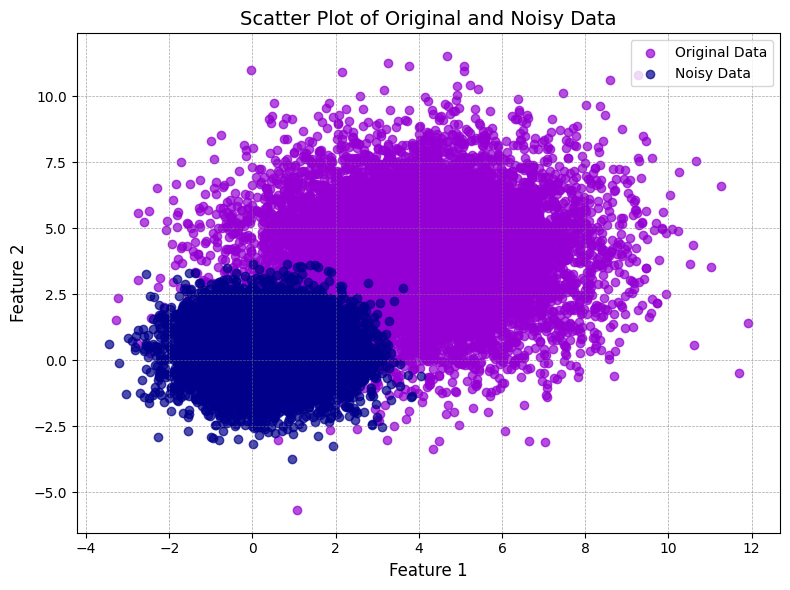
\includegraphics[width= 0.8\textwidth]{imgs/ho_implementation_init.png}
			\end{figure}
		}\only<2>{ and got satisfying results:
			\begin{figure}
				\centering
				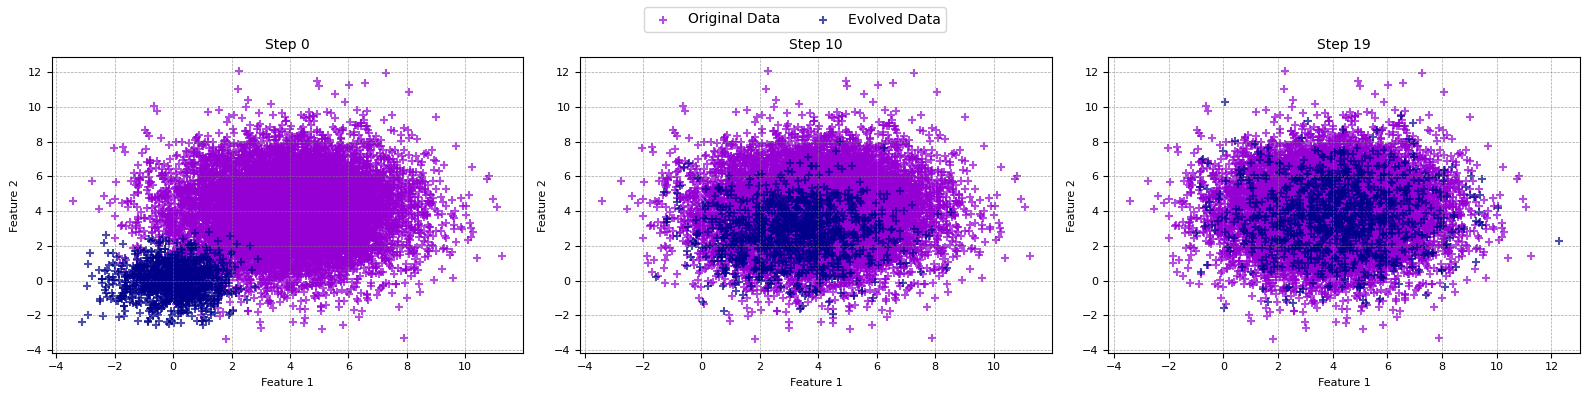
\includegraphics[width= \textwidth]{imgs/ho_gaussian_res.png}
			\end{figure}
		}
	\end{frame}
	
	\begin{frame}{Our results - Deux gaussiennes}
		
		A ajouter
		
	\end{frame}
	
	\begin{frame}{Our results - Spirale}
		Then we moved to a more complicated dataset, \alert{Spirale generation}\only<1>{:
			\begin{figure}
				\centering
				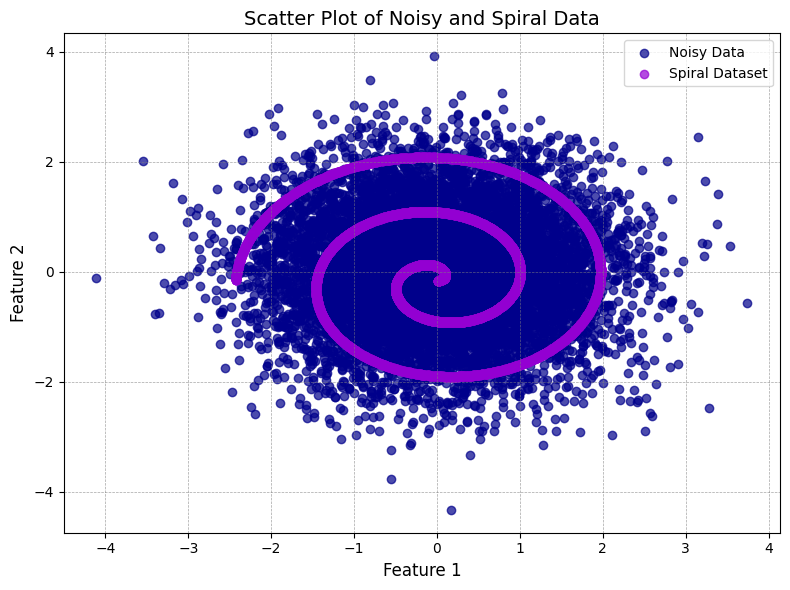
\includegraphics[width= 0.8\textwidth]{imgs/spirale_dataset.png}
		\end{figure}}\only<2>{ and also got satisfying results:
			\begin{figure}
				\centering
				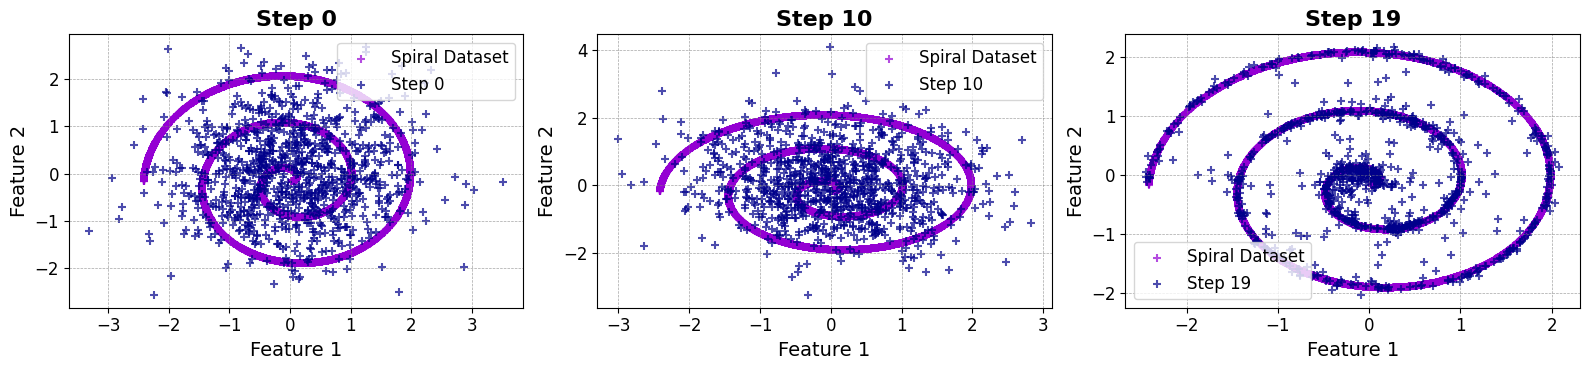
\includegraphics[width= \textwidth]{imgs/res_spirale.png}
			\end{figure}
		}
		
	\end{frame}
	
	\begin{frame}{Notre deuxième modèle - Un Unet}
		
		Ici ajouter des slides sur les Unet
		
	\end{frame}
	
	\begin{frame}{Nos résultats - MNIST}
		
		
		
	\end{frame}
	
\end{document}
